\documentclass{beamer}
\usepackage[utf8]{inputenc}

\usetheme{Madrid}
\usecolortheme{default}
\usepackage{amsmath,amssymb,amsfonts,amsthm}
\usepackage{txfonts}
\usepackage{tkz-euclide}
\usepackage{listings}
\usepackage{adjustbox}
\usepackage{array}
\usepackage{tabularx}
\usepackage{gvv}
\usepackage{lmodern}
\usepackage{circuitikz}
\usepackage{tikz}
\usepackage{graphicx}

\setbeamertemplate{page number in head/foot}[totalframenumber]

\usepackage{tcolorbox}
\tcbuselibrary{minted,breakable,xparse,skins}



\definecolor{bg}{gray}{0.95}
\DeclareTCBListing{mintedbox}{O{}m!O{}}{%
	breakable=true,
	listing engine=minted,
	listing only,
	minted language=#2,
	minted style=default,
	minted options={%
		linenos,
		gobble=0,
		breaklines=true,
		breakafter=,,
		fontsize=\small,
		numbersep=8pt,
		#1},
	boxsep=0pt,
	left skip=0pt,
	right skip=0pt,
	left=25pt,
	right=0pt,
	top=3pt,
	bottom=3pt,
	arc=5pt,
	leftrule=0pt,
	rightrule=0pt,
	bottomrule=2pt,
	toprule=2pt,
	colback=bg,
	colframe=orange!70,
	enhanced,
	overlay={%
		\begin{tcbclipinterior}
			\fill[orange!20!white] (frame.south west) rectangle ([xshift=20pt]frame.north west);
	\end{tcbclipinterior}},
	#3,
}
\lstset{
	language=C,
	basicstyle=\ttfamily\small,
	keywordstyle=\color{blue},
	stringstyle=\color{orange},
	commentstyle=\color{green!60!black},
	numbers=left,
	numberstyle=\tiny\color{gray},
	breaklines=true,
	showstringspaces=false,
}
%------------------------------------------------------------
%This block of code defines the information to appear in the
%Title page
\title %optional
{1.10.2}
%\subtitle{A short story}

\author % (optional)
{RAVULA SHASHANK REDDY - EE25BTECH11047}

 \begin{document}
	
	
	\frame{\titlepage}
	\begin{frame}{Question}
		Find the unit vector in the direction of the sum of the vectors
$\vec{a} = 2\hat{i} - \hat{j} + \hat{k}$, 
$\vec{b} = 2\hat{j} + \hat{k}$.\\

	\end{frame}
	\begin{frame}{allowframebreaks}
		\frametitle{Equation}
	\textbf{The formula for unit vector of $\vec{x}$ is : }
		\centering
		
		\label{tab:parameters}
		\begin{align*}
			\frac{\vec{x}}{\|\vec{x}||} 
		\end{align*}
		\end{frame}	
	
	\begin{frame}{Theoretical Solution}
Given :
\begin{align}
\vec{a} = \myvec{ 2 \\ -1 \\ 1 }\\ 
\vec{b} = \myvec{ 0 \\ 2 \\ 1 }.
\end{align}

Sum of the vectors:
\begin{align}
\vec{a}+\vec{b} = \myvec{ 2 \\ -1 \\ 1 } + \myvec{ 0 \\ 2 \\ 1 }
= \myvec{ 2 \\ 1 \\ 2 }.
\end{align}

Norm of $\vec{a}+\vec{b}$ :
\begin{align}
\|\vec{a}+\vec{b}\| = \sqrt{ \myvec{ 2 & 1 & 2 } 
\myvec{ 2 \\ 1 \\ 2 } }
= \sqrt{ 2\cdot 2 + 1\cdot 1 + 2\cdot 2 }
= \sqrt{9} = 3.
\end{align}
\end{frame}
\begin{frame}
Using the unit vector formula :
\begin{align}
\vec{u} = \frac{\vec{a}+\vec{b}}{\|\vec{a}+\vec{b}\|}\\
\vec{u}= \frac{1}{3} \myvec{ 2 \\ 1 \\ 2 }.
\end{align}
\begin{align}
\therefore
\vec{u} = \myvec{\frac{2}{3} \\  \frac{1}{3} \\ \frac{2}{3} }
\end{align}

\end{frame}
\begin{frame}[fragile]
		\frametitle{C Code - Unit vector function }
		
		\begin{lstlisting}

    #include <stdio.h>
#include <math.h>

// Function to compute unit vector of (x1, x2, x3)
void unitVector(double x1, double x2, double x3, double unit[3]) {
    double mag = sqrt(x1*x1 + x2*x2 + x3*x3);  // |x|
    unit[0] = x1 / mag;
    unit[1] = x2 / mag;
    unit[2] = x3 / mag;

   }
            \end{lstlisting}
            \end{frame}
            \begin{frame}[fragile]
	\frametitle{Python Code through shared output}
	\begin{lstlisting}
#Code adapted to plot only vectors a, b, a+b and unit vector
#Released under GNU GPL
import sys
import numpy as np
import numpy.linalg as LA
import matplotlib.pyplot as plt
from mpl_toolkits.mplot3d import Axes3D

# local imports 
from libs.line.funcs import *
from libs.triangle.funcs import *
from libs.conics.funcs import circ_gen

#if using termux
import subprocess
import shlex
#end if
\end{lstlisting}
            \end{frame}
            \begin{frame}[fragile]
	\frametitle{Python Code through shared output}
	\begin{lstlisting}
# Vectors from ctypes example
a = np.array([2.0, -1.0, 1.0])
b = np.array([0.0,  2.0, 1.0])
s = a + b

# Unit vector function
def unit_vector(x):
    return x / LA.norm(x)

u_py = unit_vector(s)

# Create figure
fig = plt.figure(figsize=(8, 6))
ax = fig.add_subplot(111, projection='3d')
\end{lstlisting}
            \end{frame}
            \begin{frame}[fragile]
	\frametitle{Python Code through shared output}
	\begin{lstlisting}
# Plot vectors (from origin)
ax.quiver(0,0,0,*a,color="r",label="a")
ax.quiver(0,0,0,*b,color="g",label="b")
ax.quiver(0,0,0,*s,color="b",label="a+b")

# Plot unit vector (length = 1)
ax.quiver(0,0,0,*u_py,color="c",label="unit (Python)")

# Plot scaled unit vector (same length as s)
ax.quiver(0,0,0,*(u_py*LA.norm(s)),color="c",linestyle="dashed",label="unit scaled")

ax.set_title("Vectors a, b, a+b and Unit Vector")
ax.legend()
plt.grid()
plt.show()


\end{lstlisting}
            \end{frame}
            
\begin{frame}[fragile]
\frametitle{Python code Direct}
\begin{lstlisting}
 import numpy as np
import matplotlib.pyplot as plt
from mpl_toolkits.mplot3d import Axes3D

# Define vectors
a = np.array([2, -1, 1])
b = np.array([0, 2, 1])
result = a + b                 # a + b
unit_result = result / np.linalg.norm(result)   # unit vector

# Plot
fig = plt.figure()
ax = fig.add_subplot(111, projection='3d')
\end{lstlisting}
            \end{frame}
            
\begin{frame}[fragile]
\frametitle{Python code Direct}
\begin{lstlisting}
# Plot the resultant vector
ax.quiver(0, 0, 0, result[0], result[1], result[2], color='b', label='a+b', arrow_length_ratio=0.1)

# Plot the unit vector (scaled to length 1)
ax.quiver(0, 0, 0, unit_result[0], unit_result[1], unit_result[2], color='r', label='Unit vector', arrow_length_ratio=0.1)

# Labels
ax.set_xlim([0, 3])
ax.set_ylim([0, 3])
ax.set_zlim([0, 3])
ax.set_xlabel('X')
ax.set_ylabel('Y')
ax.set_zlabel('Z')
ax.legend()

plt.show()
\end{lstlisting}
\end{frame}

\begin{frame}{Plot}
\begin{figure}
    \centering
    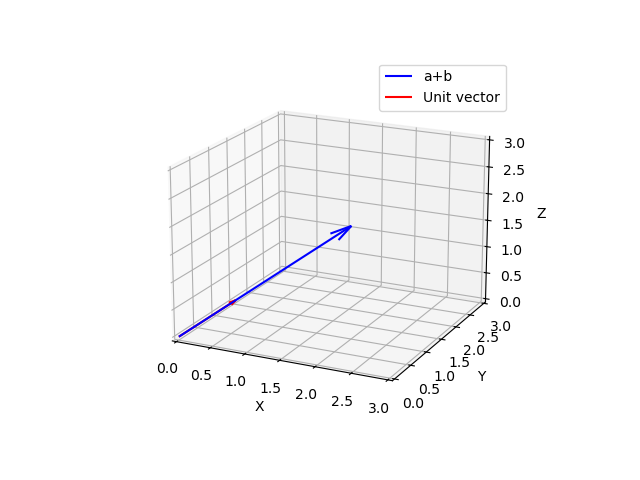
\includegraphics[width=1.0\columnwidth]{fig-1.png}
    \caption{Caption}
    \label{fig:placeholder}
\end{figure}
    
\end{frame}
\end{document}